\section{課題 2 演習ガイド}
%
%%% TERMINAL
%
\subsection{配列}
\begin{frame}[containsverbatim]
\frametitle{配列}
  \begin{itemize}
\item データオブジェクトの順序づけられた集まり
\item 配列の各オブジェクトを配列の要素と呼びます
\item 各要素は 0 から始まる自然数に対応付けられていて
\item 自然数のことをインデックスと呼んでいます
\item 各要素は配列名[インデックス]で参照することができます
  \end{itemize}
\tiny
  \begin{columns}
    \begin{column}{0.45\textwidth}
      \begin{lstlisting}[caption={単純な変数},label=naive]
d1 =  1000000000000000000000000000
d2 =  1000000000110000110000000000
d3 =  1000000000110000110000000000
d4 =  1000000000000000000000000000
d5 =  1000001100000000000011000000
d6 =  1000000110000000000110000000
d7 =  1000000011000000001100000000
d8 =  1000000000111111110000000000
d9 =  1000000000000000000000000000
      \end{lstlisting}
    \end{column}
    \begin{column}{0.45\textwidth}
      \begin{lstlisting}[caption={配列},label=array]
 d = [1000000000000000000000000000,
      1000000000110000110000000000,
      1000000000110000110000000000,
      1000000000000000000000000000,
      1000001100000000000011000000,
      1000000110000000000110000000,
      1000000011000000001100000000,
      1000000000111111110000000000,
      1000000000000000000000000000]
      \end{lstlisting}
    \end{column}
  \end{columns}
\end{frame}
\begin{frame}[containsverbatim]
\frametitle{配列の参照と代入}
  \begin{itemize}
\item 連続したメモリ領域を確保
\item 先頭を 0 としてインデックスで参照 (ここは板書します)
  \end{itemize}
\tiny
  \begin{columns}
    \begin{column}{0.5\textwidth}
      \begin{lstlisting}[caption={代入},label=array-assign]
 d = [0]*9
 d[0]=1000000000000000000000000000
 d[1]=1000000000110000110000000000
 d[2]=1000000000110000110000000000
 d[3]=1000000000000000000000000000
 d[4]=1000001100000000000011000000
 d[5]=1000000110000000000110000000
 d[6]=1000000011000000001100000000
 d[7]=1000000000111111110000000000
 d[8]=1000000000000000000000000000
      \end{lstlisting}
    \end{column}
    \begin{column}{0.35\textwidth}
      \begin{lstlisting}[caption={参照},label=array-ref]
 for i in range(9):
   print(d[i])
      \end{lstlisting}
\centering
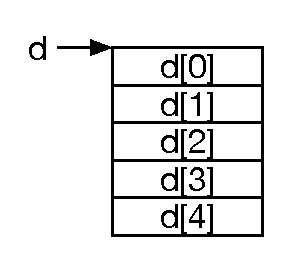
\includegraphics[scale=0.5]{./Figure/elementaryCS-figArray.eps}
    \end{column}
  \end{columns}
\end{frame}
\begin{frame}[containsverbatim]
\frametitle{配列の例}
  \begin{itemize}
\item 総和を求める
\item \lstref{lst:sum6}: 整数の配列を宣言する例
\item \lstref{lst:sum}: 入力した整数を配列にする例
  \end{itemize}
  \begin{columns}
    \begin{column}{0.35\textwidth}
      \begin{lstlisting}[caption={総和},label=lst:sum6]
a=[2,4,6,8,10,12]
s=0
for k in range(len(a)):
  s=s+a[k]
  k=k+1
print(s)
      \end{lstlisting}
    \end{column}
    \begin{column}{0.6\textwidth}
      \begin{lstlisting}[caption=入力した数の総和,label=lst:sum]
a = list(map(int,input("numbers? ").split()))
s=0
for k in range(len(a)):
  s=s+a[k]
  k=k+1
print(s)
      \end{lstlisting}
    \end{column}
  \end{columns}
\end{frame}
\begin{frame}[containsverbatim, shrink]
\frametitle{最大値を求める}
\framesubtitle{宿題 2}
  \begin{itemize}
\item \href{https://sites.google.com/a/presystems.xyz/sample/home/elementary-computer-science}{\beamerbutton{https://sites.google.com/a/presystems.xyz/sample/home/elementary-computer-science}} の max-skeleton.py を完成させる
\item 最大値=max\((a_1, a_2,\cdots,a_n)\)
\item {\tt for j in range(0,n)} は {\tt j} を 0 から n-1 まで繰り返すという意味
  \end{itemize}
\vspace{-1em}
  \begin{columns}
    \begin{column}{0.6\textwidth}
      \begin{lstlisting}[caption={max.py},label=lst:max]
# max.py
# 入力: 整数の列
# 出力: 最大値
array = list(map(int,input("numbers? ").split()))
if not array:  # array が空の場合
    raise ValueError("...")  # 入力エラー
# 以下が計算部分
max_value = array[0]      # array[0] を一時的に最大値に
max_index = 0
for i in range(0,(len(array))):
  if :                    # より大きな数を探す
    max_value =
    max_index =
print(max_value, max_index)
      \end{lstlisting}
    \end{column}
    \begin{column}{0.35\textwidth}
      \begin{itembox}{出力例}
\scriptsize
> python3 max.py\\
numbers? -3 8 19 -4\\
19 2
      \end{itembox}
    \end{column}
  \end{columns}
\end{frame}
%
%%% STRINGS
%
\subsection{文字列}
\begin{frame}
\frametitle{文字データの表現}
  \begin{itemize}
\item コンピュータは数値だけでなく文字も処理することができる
\item 文字はコード化されて処理される
\item 文字列は文字の配列
  \end{itemize}
\end{frame}
\begin{frame}
\frametitle{文字コード}
  \begin{itemize}
\item コードとは,文字や記号をコンピュータで扱うための記号です
\item コンピュータ内では適当な正整数が文字や記号に割り振られています
    \begin{itemize}
\item 整数は 2 進数で表されているので 0 と 1 の列にコード化されます
    \end{itemize}
\item コードは任意に決めることもできます
\item しかし,各コンピュータで違っていては不都合が生じます
\item 異なるコンピュータでは全く違った文字になってしまうかも知れません
    \begin{itemize}
\item 文字コードが違っているとうまく表示できません
    \end{itemize}
  \end{itemize}
\end{frame}
\begin{frame}
\frametitle{コードの違いの例}
  \begin{itemize}
\item 3 という文字のコードの例です
\item 下の図は電光掲示板の例です
\item 左の図では 110 1110$_{(2)}$ とコードを割り当てています
\item 右の図では 111 1100$_{(2)}$ とコードを割り当てています
\item このように違ったコードを対応づけることもできます
  \end{itemize}
  \begin{example}[電光掲示板の例]
    \begin{center}
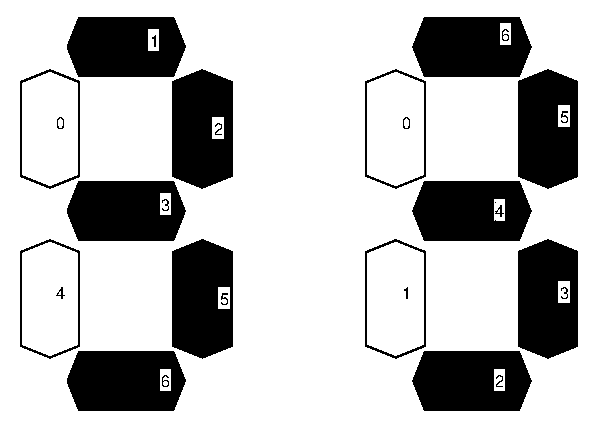
\includegraphics[scale=0.5]{./Figure/ComputerLiteracy-figThree.eps}
    \end{center}
  \end{example}
\end{frame}
\begin{frame}
\frametitle{ASCII コード}
  \begin{itemize}
\item 共通のコード体系として ASCII コードが策定されました
\item これは英語のアルファベットと数字と記号にコードを割り当てています
    \begin{itemize}
\item \href{https://en.wikipedia.org/wiki/ASCII\#/media/File:US-ASCII\_code\_chart.png}{\beamerbutton{ASCII Code Chart}}
    \end{itemize}
  \end{itemize}
\end{frame}
\begin{frame}
\frametitle{日本語漢字のコード体系}
  \begin{itemize}
\item 現在は日本語など漢字圏の文字もコードが割り当てられています
\item JIS, Shift-JIS, EUC, Unicode があります
    \begin{itemize}
\item これらは異なるコード体系です
\item 同じ文字でも異なるコードが割り当てられています
    \end{itemize}
\item 漢字圏で Unicode 以前に用いていたコードの規格
    \begin{itemize}
\item 日本: JIS X 0208-1990, JIS X 0212-1990(第一水準,第二水準,補助漢字)
\item 中国: GB 2312-80, GB 12345-90$\cdots$
\item 台湾: CNS 111643-1986
\item 韓国: KS C 5601-1987, KS C 5657-1991
    \end{itemize}
\item Python3 は Unicode を利用しています
  \end{itemize}
\end{frame}
\begin{frame}[containsverbatim, shrink]
\frametitle{Python での文字列}
  \begin{itemize}
\item 文字列は各文字の配列として扱える
\item {\texttt str} という名前の配列の各要素に一文字入っている
\item 0 番目から順番にインデックスで参照できる
  \end{itemize}
  \begin{columns}
    \begin{column}{0.55\textwidth}
      \begin{lstlisting}[caption={stringPrint.py},label=lst:strprt]
# stringPrint.py
# 文字列処理の練習プログラム
# 入力: 文字列
# 出力: 文字列の文字を1行1文字で出す
import os

os.system('clear')
str = (input("strings? ")).encode("ascii")
print(str)
for k in range(0,len(str)):
   print(chr(str[k]), hex(str[k]))
      \end{lstlisting}
    \end{column}
    \begin{column}{0.35\textwidth}
      \begin{itembox}{出力例}
\scriptsize
> python3 stringPrint.py\\
strings? Ice\%cream\\
I 0x49\\
c 0x63\\
e 0x65\\
\% 0x25\\
c 0x63\\
r 0x72\\
e 0x65\\
a 0x61\\
m 0x6d
      \end{itembox}
    \end{column}
  \end{columns}
\end{frame}
\begin{frame}[containsverbatim]
\frametitle{文字列の表現}
  \begin{itemize}
\item 文字列は文字の配列
\item 各文字はその符号(文字コード)で表されて
\item 各要素に各文字コードを格納
  \end{itemize}
  \begin{columns}
    \begin{column}{0.4\textwidth}
      \begin{itembox}{出力例}
\scriptsize
> python3 stringPrint.py\\
strings? Ice\%cream\\
I 0x49\\
c 0x63\\
e 0x65\\
\% 0x25\\
c 0x63\\
r 0x72\\
e 0x65\\
a 0x61\\
m 0x6d
      \end{itembox}
    \end{column}
    \begin{column}{0.6\textwidth}
      \begin{center}
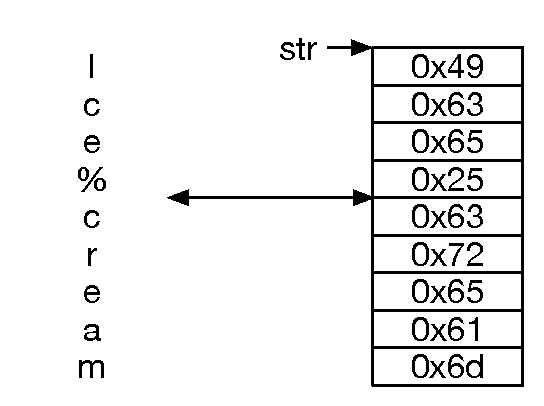
\includegraphics[scale=0.5]{./Figure/elementaryCS-figStrings.eps}
      \end{center}
    \end{column}
  \end{columns}
\end{frame}
\begin{frame}[containsverbatim, shrink]
\frametitle{英小文字だけを画面に出力}
\framesubtitle{宿題 3}
  \begin{itemize}
\item \href{https://sites.google.com/a/presystems.xyz/sample/home/elementary-computer-science}{\beamerbutton{https://sites.google.com/a/presystems.xyz/sample/home/elementary-computer-science}} の abcPrint-skeleton.py を完成させる
  \end{itemize}
  \begin{columns}
    \begin{column}{0.6\textwidth}
      \begin{lstlisting}[caption={abcPrint.py},label=lst:lowerletterprt]
# abcPrint.py
# 文字列処理の練習プログラム,小文字だけ出力
# 入力: 文字列
# 出力: 文字列の文字で小文字のみ出力する
ss = (input("strings? ")).encode("ascii")
for k, code in enumerate(ss):
  if :                   # 小文字ならば
     print(chr(ss[k]))   # 文字を表示する
      \end{lstlisting}
    \end{column}
    \begin{column}{0.35\textwidth}
      \begin{itembox}{出力例}
\scriptsize
> python3 abcPrint.py\\
strings? Ice\%cream\\
c\\
e\\
c\\
r\\
e\\
a\\
m
      \end{itembox}
    \end{column}
  \end{columns}
\end{frame}
%
%%% QUIZ 2
%
\subsection{課題 2 予告}
\begin{frame}
\frametitle{課題 2 予告}
  \begin{itemize}
\item 来週の予定です
\item \hyperlink{quiz2}{\beamerbutton{Jump to Quiz 2}}
  \end{itemize}
\end{frame}
